
This section contains exploring notions of structured sparsity. We will further develop some ideas useful to the study of tree-decompositions and degeneracy.

\subsection{Minor subgraphs}\label{sec:minors}

As usual, all graphs we consider here are standard graphs.
Recall that a graph $G$ contains $H$ as a \emph{minor subgraph} (also called simply ``a minor") if you can obtain a copy of $H$ by a sequence of node deletions, edge deletions, and edge contractions (defined below).
We will later describe important variations on this idea (e.g. ``shallow" and ``topological" minor subgraphs), but first we want to make clear the importance of subgraph minors to the study of sparsity.

We will illustrate the connection of minors to sparsity with an example.
One canonical example of ``sparse" graphs are the family of planar graphs -- planar graphs have $O(n)$ edges and bounded degeneracy.
It turns out that planar graphs are completely characterized by subgraph minors.
To elaborate: a graph $G$ is planar if and only if $G$ does not contains $K_5$ or $K_{3,3}$ as minors (where $K_5$ is the complete graph on 5 nodes, and $K_{3,3}$ is the complete-bipartite graph with 3 nodes in each partition).
This is an example of a type of sparsity that is completely characterized by specific graph minors.

The point here is that having knowledge of the minors of a graph can help determine the sparsity of the graph.
Therefore, we would like an easy way to learn some information about the minors of a graph.
We are not aiming to characterize any graph family completely (that is a little ambitious); rather, our goal is to try to reveal connections between a graph's eigenproperties and a graph's minors.


\subsubsection{Terminology}

%topological minors, and $r$-shallow minors
\paragraph{Operations}

To perform an \emph{edge contraction} on an edge with endpoints $v_1, v_2$, create a new node $v$, attached an edge from $v$ to each neighbor of $v_1$ and each neighbor of $v_2$, then delete nodes $v_1$ and $v_2$. You can think of this as merging the two nodes $v_1, v_2$ into each other.

\begin{figure}[h!]
  \centering
  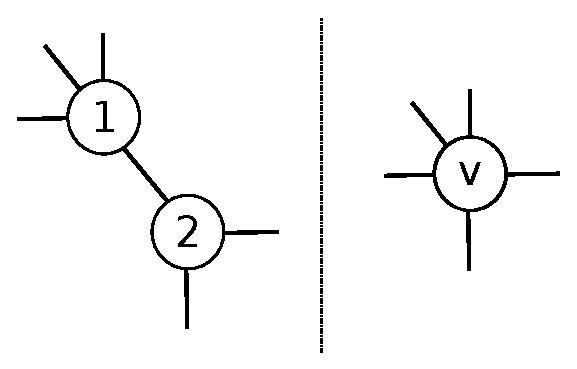
\includegraphics[scale=0.75]{edge-contraction}
  \caption{(\emph{Left}.) Nodes $v_1$ and $v_2$ connected by an edge. (\emph{Right}.) The graph after contracting edge $v_1v_2$, merging nodes $v_1$ and $v_2$ into one new node, $v$.\label{fig:contracting}}
\end{figure}

A \emph{subdivision} (or ``edge subdivision") is sort of the reverse of an edge contraction: given an edge with endpoints $v_1, v_2$, to subdivide the edge $e_{12}$, create a new node $v$, connect $v$ with an edge to node $v_1$ and an edge to $v_2$, then delete edge $e_{12}$. This operation is like spitting edge $e_{12}$ into two pieces connected by a new node $v$. Note that a subdivision introduces a node of degree two. The reverse process, ``un-subdividing", is called \emph{smoothing} or \emph{dissolving} a node of degree two. If node $v$ has degree two and is connected to nodes $v_1$ and $v_2$, then smoothing node $v$ is performed by connecting node $v_1$ and $v_2$ with an edge, then deleting node $v$. See Figure~\ref{fig:smoothing} for an illustration. Smoothing a node of degree two can also be thought of as an edge-contraction on either of the edges touching the node.

\begin{figure}[h!]
  \centering
  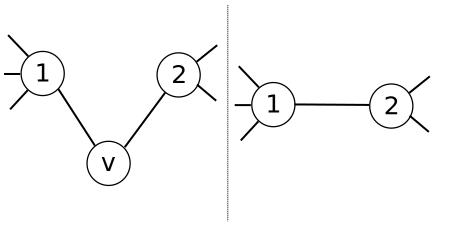
\includegraphics[scale=0.75]{smoothing}
  \caption{(\emph{Left}.) Nodes $v_1$ and $v_2$ separated by a node of degree two, $v$. (\emph{Right}.) The graph after node $v$ has been smoothed; alternatively, this can be understood as contracting edge $v_1v$ or edge $v_2v$.
  Note that viewing the figure from right to left gives an illustration of the edge between $v_1$ and $v_2$ being subdivided.\label{fig:smoothing}}
\end{figure}

A graph $T$ is a \emph{topological minor} of $G$ if you can produce $G$ from $T$ by subdividing edges of $T$, and adding nodes and edges to $T$. Put another way, $T$ is a topological minor (``top-minor" for short) of $G$ if you can produce $T$ from $G$ by deleting nodes and edges, and smoothing nodes (of degree two). Note that all topological minor subgraphs are also minor subgraphs. See Figure~\ref{fig:topminor} for an example of a graph with a $K_4$ as a topological minor.
For contrast, Figure~\ref{fig:minorsubg} displays a graph that does not contain $K_5$ as a subgraph or as a topological minor subgraph (no node has degree 2, so no nodes can be smoothed), but it does contain $K_5$ as a minor subgraph.

\begin{figure}[h!]
  \centering
  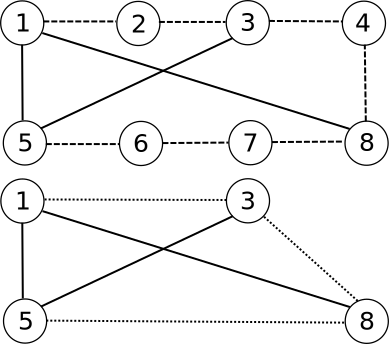
\includegraphics[scale=0.8]{topminor}
  \caption{ In the top graph, smoothing the nodes connected to only dashed egdes yields the graph on bottom as a topological minor. Alternatively, this can be thought of as contracting the dashed edges.
  Note that the dotted edges in the bottom graph indicate the edges produced by the smoothings in the top graph. Finally, viewing this figure from bottom to top, this illustrates an instance of $K_4$ where we then perform several subdivisions on the dotted edges to produce the graph on top.\label{fig:topminor}}
\end{figure}

\begin{figure}[h!]
  \centering
  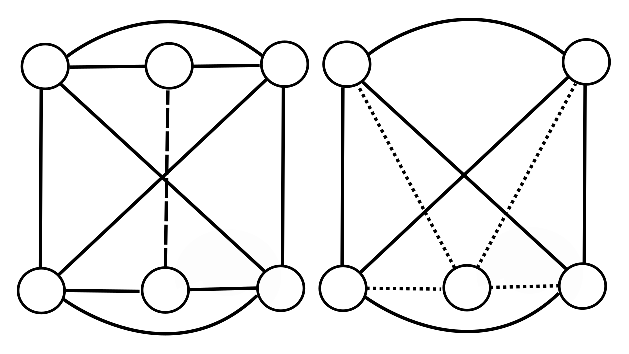
\includegraphics[scale=0.8]{minorsubg}
  \caption{ (\emph{Left}.) This graph does not contain $K_5$ as a subgraph, or as a topological minor subgraph. (\emph{Right}.) Contracting the dashed edge on the left yields a new node, with new dotted edges in the graph on the right. The graph on the right is $K_5$, so this proves the graph on the left has $K_5$ as a minor subgraph.\label{fig:minorsubg}}
\end{figure}

Finally, this brings us to the notion of ``shallowness" of minor subgraphs. Minor subgraphs are used, among other things, for measuring ``density" of a given graph $G$ --- ``$G$ is not sparse" can mean ``$G$ has no dense minor subgraphs like $K_n$". But this notion of measuring density (by looking for the presence of a particular kind of minor subgraph) isn't always precise if, for example, you have to contract a whole lot of sparse components of the graph to be able to produce a ``dense" minor subgraph. The concept of shallowness measures this idea: ``how much contracting must I perform before the result starts to look dense?". We illustrate with an example.

Fix some $n$ and consider $G = K_n$, the complete graph on $n$ nodes; this is the densest graph there is (on $n$ nodes). Now suppose pick one edge and subdivide that edge $c$ times to produce $G'$. There are $\binom{n}{2}$ edges in $G$, so there are $c + \binom{n}{2}$ total edges in $G'$. The graph $G'$ also now has $n+c$ nodes. Is this graph still dense? As we increase $c$ to infinity, $G'$ looks less like ``$G$ with a few extra edges" and more like "one long path graph with a tiny cluster tacked onto its end". Regardless of $c$, the graph $G'$ has $K_n$ as a minor subgraph. But the larger $c$ is, the more contracting must be performed on $G'$ to attain $K_n$ --- the less shallow $K_n$ becomes as a minor subgraph of $G'$.




\begin{tabular}[h]{lcl}
  \\
  object & & operations allowed \\
  \toprule
  minor subgraph & & node deletions \\
    & & edge deletions \\
    & & edge contractions \\
  topological minor subgraph & & node deletions \\
  & & edge deletions \\
  & & node smoothings (contracting edges touching a node of degree 2)\\
  $r$-shallow minor & & node deletions \\
   & & edge deletions \\
   & & ``not more than $r$ edge contractions at each node"\\
\end{tabular}
